\documentclass{standalone}
\usepackage{pgfplots}
\usepgfplotslibrary{patchplots}
\begin{document}
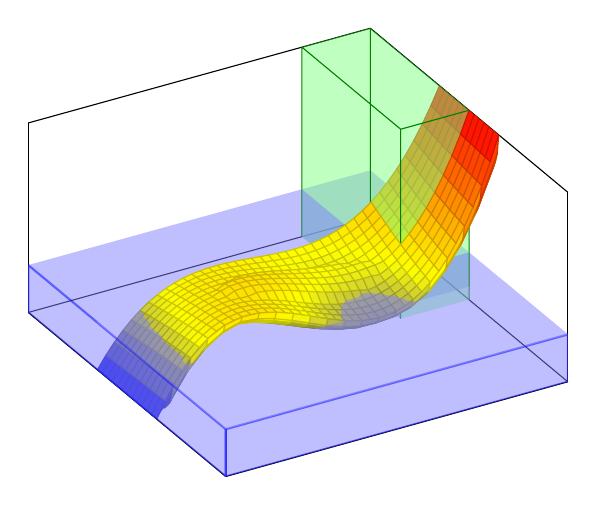
\begin{tikzpicture}

\begin{axis}[
   %xlabel=x,
   %ylabel=y,
   xmin=0, xmax=1,
   ymin=0, ymax=1,
   zmin=0, zmax=1,
   xtick=\empty, ytick=\empty, ztick=\empty,
   view={-30}{45},
   %view={0}{0},
   ]

   \fill[blue!50,opacity=0.5,even odd rule]
(axis cs:0,0,0.25) -- (axis cs:1,0,0.25) -- (axis cs:1,1,0.25) -- (axis cs:0,1,0.25) -- cycle
(axis cs:0.0,0.655,0.25) -- (axis cs:0.01,0.655,0.25) -- (axis cs:0.02,0.655,0.25) -- (axis cs:0.03,0.655,0.25) -- (axis cs:0.04,0.655,0.25) -- (axis cs:0.05,0.655,0.25) -- (axis cs:0.06,0.655,0.25) -- (axis cs:0.07,0.655,0.25) -- (axis cs:0.08,0.655,0.25) -- (axis cs:0.09,0.655,0.25) -- (axis cs:0.1,0.655,0.25) -- (axis cs:0.11,0.655,0.25) -- (axis cs:0.12,0.655,0.25) -- (axis cs:0.125,0.65,0.25) -- (axis cs:0.125,0.64,0.25) -- (axis cs:0.125,0.63,0.25) -- (axis cs:0.12,0.625,0.25) -- (axis cs:0.115,0.62,0.25) -- (axis cs:0.115,0.61,0.25) -- (axis cs:0.115,0.6,0.25) -- (axis cs:0.115,0.5900000000000001,0.25) -- (axis cs:0.115,0.5800000000000001,0.25) -- (axis cs:0.11,0.575,0.25) -- (axis cs:0.105,0.5700000000000001,0.25) -- (axis cs:0.105,0.56,0.25) -- (axis cs:0.105,0.55,0.25) -- (axis cs:0.105,0.54,0.25) -- (axis cs:0.105,0.53,0.25) -- (axis cs:0.105,0.52,0.25) -- (axis cs:0.105,0.51,0.25) -- (axis cs:0.105,0.5,0.25) -- (axis cs:0.1,0.495,0.25) -- (axis cs:0.095,0.49,0.25) -- (axis cs:0.095,0.48,0.25) -- (axis cs:0.095,0.47,0.25) -- (axis cs:0.095,0.45999999999999996,0.25) -- (axis cs:0.095,0.44999999999999996,0.25) -- (axis cs:0.095,0.43999999999999995,0.25) -- (axis cs:0.095,0.43000000000000005,0.25) -- (axis cs:0.095,0.42000000000000004,0.25) -- (axis cs:0.095,0.41000000000000003,0.25) -- (axis cs:0.095,0.4,0.25) -- (axis cs:0.095,0.39,0.25) -- (axis cs:0.095,0.38,0.25) -- (axis cs:0.09,0.375,0.25) -- (axis cs:0.085,0.37,0.25) -- (axis cs:0.085,0.36,0.25) -- (axis cs:0.085,0.35,0.25) -- (axis cs:0.09,0.345,0.25) -- (axis cs:0.1,0.345,0.25) -- (axis cs:0.11,0.345,0.25) -- (axis cs:0.12,0.345,0.25) -- (axis cs:0.13,0.345,0.25) -- (axis cs:0.14,0.345,0.25) -- (axis cs:0.15,0.345,0.25) -- (axis cs:0.16,0.345,0.25) -- (axis cs:0.17,0.345,0.25) -- (axis cs:0.18,0.345,0.25) -- (axis cs:0.19,0.345,0.25) -- (axis cs:0.2,0.345,0.25) -- (axis cs:0.21,0.345,0.25) -- (axis cs:0.22,0.345,0.25) -- (axis cs:0.23,0.345,0.25) -- (axis cs:0.24,0.345,0.25) -- (axis cs:0.25,0.345,0.25) -- (axis cs:0.26,0.345,0.25) -- (axis cs:0.27,0.345,0.25) -- (axis cs:0.28,0.345,0.25) -- (axis cs:0.29,0.345,0.25) -- (axis cs:0.3,0.345,0.25) -- (axis cs:0.31,0.345,0.25) -- (axis cs:0.32,0.345,0.25) -- (axis cs:0.33,0.345,0.25) -- (axis cs:0.34,0.345,0.25) -- (axis cs:0.35,0.345,0.25) -- (axis cs:0.36,0.345,0.25) -- (axis cs:0.37,0.345,0.25) -- (axis cs:0.38,0.345,0.25) -- (axis cs:0.39,0.345,0.25) -- (axis cs:0.4,0.345,0.25) -- (axis cs:0.41,0.345,0.25) -- (axis cs:0.42,0.345,0.25) -- (axis cs:0.43,0.345,0.25) -- (axis cs:0.44,0.345,0.25) -- (axis cs:0.45,0.345,0.25) -- (axis cs:0.46,0.345,0.25) -- (axis cs:0.47,0.345,0.25) -- (axis cs:0.48,0.345,0.25) -- (axis cs:0.49,0.345,0.25) -- (axis cs:0.5,0.345,0.25) -- (axis cs:0.51,0.345,0.25) -- (axis cs:0.52,0.345,0.25) -- (axis cs:0.53,0.345,0.25) -- (axis cs:0.54,0.345,0.25) -- (axis cs:0.545,0.35,0.25) -- (axis cs:0.545,0.36,0.25) -- (axis cs:0.55,0.365,0.25) -- (axis cs:0.555,0.37,0.25) -- (axis cs:0.555,0.38,0.25) -- (axis cs:0.56,0.385,0.25) -- (axis cs:0.565,0.39,0.25) -- (axis cs:0.565,0.4,0.25) -- (axis cs:0.57,0.405,0.25) -- (axis cs:0.575,0.41000000000000003,0.25) -- (axis cs:0.58,0.41500000000000004,0.25) -- (axis cs:0.585,0.42000000000000004,0.25) -- (axis cs:0.59,0.42500000000000004,0.25) -- (axis cs:0.595,0.43000000000000005,0.25) -- (axis cs:0.6,0.43500000000000005,0.25) -- (axis cs:0.61,0.43500000000000005,0.25) -- (axis cs:0.62,0.43500000000000005,0.25) -- (axis cs:0.63,0.43500000000000005,0.25) -- (axis cs:0.64,0.43500000000000005,0.25) -- (axis cs:0.645,0.43999999999999995,0.25) -- (axis cs:0.65,0.44499999999999995,0.25) -- (axis cs:0.66,0.44499999999999995,0.25) -- (axis cs:0.67,0.44499999999999995,0.25) -- (axis cs:0.675,0.43999999999999995,0.25) -- (axis cs:0.68,0.43500000000000005,0.25) -- (axis cs:0.685,0.43000000000000005,0.25) -- (axis cs:0.69,0.42500000000000004,0.25) -- (axis cs:0.695,0.42000000000000004,0.25) -- (axis cs:0.7,0.41500000000000004,0.25) -- (axis cs:0.705,0.41000000000000003,0.25) -- (axis cs:0.71,0.405,0.25) -- (axis cs:0.715,0.4,0.25) -- (axis cs:0.72,0.395,0.25) -- (axis cs:0.725,0.39,0.25) -- (axis cs:0.725,0.38,0.25) -- (axis cs:0.73,0.375,0.25) -- (axis cs:0.735,0.37,0.25) -- (axis cs:0.735,0.36,0.25) -- (axis cs:0.74,0.355,0.25) -- (axis cs:0.745,0.35,0.25) -- (axis cs:0.75,0.345,0.25) -- (axis cs:0.76,0.345,0.25) -- (axis cs:0.77,0.345,0.25) -- (axis cs:0.78,0.345,0.25) -- (axis cs:0.79,0.345,0.25) -- (axis cs:0.8,0.345,0.25) -- (axis cs:0.81,0.345,0.25) -- (axis cs:0.82,0.345,0.25) -- (axis cs:0.83,0.345,0.25) -- (axis cs:0.84,0.345,0.25) -- (axis cs:0.85,0.345,0.25) -- (axis cs:0.86,0.345,0.25) -- (axis cs:0.87,0.345,0.25) -- (axis cs:0.88,0.345,0.25) -- (axis cs:0.89,0.345,0.25) -- (axis cs:0.9,0.345,0.25) -- (axis cs:0.91,0.345,0.25) -- (axis cs:0.92,0.345,0.25) -- (axis cs:0.93,0.345,0.25) -- (axis cs:0.94,0.345,0.25) -- (axis cs:0.95,0.345,0.25) -- (axis cs:0.96,0.345,0.25) -- (axis cs:0.97,0.345,0.25) -- (axis cs:0.98,0.345,0.25) -- (axis cs:0.99,0.345,0.25) -- (axis cs:1.0,0.345,0.25) -- (axis cs:1.0,0.0,0.25) -- (axis cs:0.0,0.0,0.25) -- cycle
;


   % top of RxO (back, positive y half, in green box)
   \addplot3[
           surf,
           opacity = 1.0,
           samples=9,
           samples y=7,
           domain=0.8:1.0,y domain=0:1,
           z buffer=sort]
       ({x},
        {(0.5+0.15*(y))},
        {((8*x^3 - 11*x^2 + 4*x)*(1-(0.5+0.15*(y))^2) + (x)*((0.5+0.15*(y))^2)) + 0.05*(max(0.00001,1-(2*y)^2-2*(3*(x-0.5))^2))^0.5});

   % RxRE side surface (domain is z)
   %\addplot3[
   %   surf,green!50!white,faceted color=green!30!black,
   %   opacity=0.5,
   %   samples=21,samples y=21,
   %   domain=0:1,y domain=0.5:1.0,
   %   z buffer=sort]
   %   ({0.8}, {y}, {x});
   \fill[green!50,opacity=0.5]
      (axis cs:0.8,1.0,1.0) -- (axis cs:0.8,0.5,1.0) -- (axis cs:0.8,0.5,0.0) -- (axis cs:0.8,1.0,0.0) -- cycle;
   % RxRE front surface (domain is z)
   %\addplot3[
   %   surf,green!50!white,faceted color=green!50!black,
   %   opacity=0.5,
   %   samples=21,samples y=9,
   %   domain=0:1,y domain=0.8:1.0,
   %   z buffer=sort]
   %   ({y}, {0.5}, {x});
   \fill[green!50,opacity=0.5]
      (axis cs:0.8,0.5,1.0) -- (axis cs:1.0,0.5,1.0) -- (axis cs:1.0,0.5,0.0) -- (axis cs:0.8,0.5,0.0) -- cycle;
   % RxRE top surface
   %\addplot3[
   %   surf,green!50!white,faceted color=green!50!black,
   %   opacity=0.5,
   %   samples=9,samples y=21,
   %   domain=0.8:1,y domain=0.5:1.0,
   %   z buffer=sort]
   %   ({x}, {y}, {1.0});
   \fill[green!50,opacity=0.5]
      (axis cs:0.8,1.0,1.0) -- (axis cs:1.0,1.0,1.0) -- (axis cs:1.0,0.5,1.0) -- (axis cs:0.8,0.5,1.0) -- cycle;
   % add lines (top)
   %\draw[green!50!black] ;
   % add lines (sides)
   \draw[green!50!black]
      (axis cs:0.8,1.0,1.0) -- (axis cs:1.0,1.0,1.0) -- (axis cs:1.0,0.5,1.0) -- (axis cs:0.8,0.5,1.0) -- cycle
      (axis cs:0.8,1.0,0.0) -- (axis cs:0.8,1.0,1.0)
      (axis cs:1.0,1.0,0.0) -- (axis cs:1.0,1.0,1.0)
      (axis cs:0.8,0.5,0.0) -- (axis cs:0.8,0.5,1.0)
      (axis cs:1.0,0.5,0.0) -- (axis cs:1.0,0.5,1.0);

   % fix up side/front surfaces with transparent blue
   \fill[blue!50,opacity=0.5]
      (axis cs:0.8,1,0) -- (axis cs:0.8,1,0.25) -- (axis cs:0.8,0.5,0.25) -- (axis cs:0.8,0.5,0) -- cycle;
   \fill[blue!50,opacity=0.5]
      (axis cs:0.8,0.5,0.07) -- (axis cs:0.8,0.5,0.25) -- (axis cs:1.0,0.5,0.25) -- (axis cs:1.0,0.5,0.07) -- cycle;

   % bottom of RxO (front, negative y half only)
   \addplot3[
           surf,
           opacity = 1.0,
           samples=21,
           samples y=21,
           domain=0:1,y domain=-1:0,
           z buffer=sort]
       ({x},
        {(0.5+0.15*(y))},
        {max(0.0, ((8*x^3 - 11*x^2 + 4*x)*(1-(0.5+0.15*(y))^2) + (x)*((0.5+0.15*(y))^2))
           - (0.1 + 0.04*abs(24*x^2 -22*x + 4))*max(0.00001,(1-y^2))^0.5)});

   % top of RxO (back, positive y half)
   \addplot3[
           surf,
           opacity = 1.0,
           samples=33,
           samples y=7,
           domain=0:0.8,y domain=0:1,
           z buffer=sort]
       ({x},
        {(0.5+0.15*(y))},
        {((8*x^3 - 11*x^2 + 4*x)*(1-(0.5+0.15*(y))^2) + (x)*((0.5+0.15*(y))^2)) + 0.05*(max(0.00001,1-(2*y)^2-2*(3*(x-0.5))^2))^0.5});

   % top of RxO (front, negative y half)
   \addplot3[
           surf,
           opacity = 1.0,
           samples=41,
           samples y=7,
           domain=0:1,y domain=-1:0,
           z buffer=sort]
       ({x},
        {(0.5+0.15*(y))},
        {((8*x^3 - 11*x^2 + 4*x)*(1-(0.5+0.15*(y))^2) + (x)*((0.5+0.15*(y))^2)) + 0.05*(max(0.00001,1-(2*y)^2-2*(3*(x-0.5))^2))^0.5});

   % draw lower box
   % front
   \draw[thick,blue,fill=blue!50,opacity=0.5]
      (axis cs:0,0,0) -- (axis cs:0,0,0.25) -- (axis cs:1,0,0.25) -- (axis cs:1,0,0.0) -- cycle;
   % side (left)
   \draw[thick,blue,fill=blue!50,opacity=0.5]
      (axis cs:0,0,0) -- (axis cs:0,0,0.25) -- (axis cs:0,1,0.25) -- (axis cs:0,1,0.0) -- cycle;

   % this does even odd rule
   \fill[blue!50,opacity=0.5,even odd rule]
(axis cs:0.0,0.655,0.25) -- (axis cs:0.01,0.655,0.25) -- (axis cs:0.02,0.655,0.25) -- (axis cs:0.03,0.655,0.25) -- (axis cs:0.04,0.655,0.25) -- (axis cs:0.05,0.655,0.25) -- (axis cs:0.06,0.655,0.25) -- (axis cs:0.07,0.655,0.25) -- (axis cs:0.08,0.655,0.25) -- (axis cs:0.09,0.655,0.25) -- (axis cs:0.1,0.655,0.25) -- (axis cs:0.11,0.655,0.25) -- (axis cs:0.12,0.655,0.25) -- (axis cs:0.125,0.65,0.25) -- (axis cs:0.125,0.64,0.25) -- (axis cs:0.125,0.63,0.25) -- (axis cs:0.12,0.625,0.25) -- (axis cs:0.115,0.62,0.25) -- (axis cs:0.115,0.61,0.25) -- (axis cs:0.115,0.6,0.25) -- (axis cs:0.115,0.5900000000000001,0.25) -- (axis cs:0.115,0.5800000000000001,0.25) -- (axis cs:0.11,0.575,0.25) -- (axis cs:0.105,0.5700000000000001,0.25) -- (axis cs:0.105,0.56,0.25) -- (axis cs:0.105,0.55,0.25) -- (axis cs:0.105,0.54,0.25) -- (axis cs:0.105,0.53,0.25) -- (axis cs:0.105,0.52,0.25) -- (axis cs:0.105,0.51,0.25) -- (axis cs:0.105,0.5,0.25) -- (axis cs:0.1,0.495,0.25) -- (axis cs:0.095,0.49,0.25) -- (axis cs:0.095,0.48,0.25) -- (axis cs:0.095,0.47,0.25) -- (axis cs:0.095,0.45999999999999996,0.25) -- (axis cs:0.095,0.44999999999999996,0.25) -- (axis cs:0.095,0.43999999999999995,0.25) -- (axis cs:0.095,0.43000000000000005,0.25) -- (axis cs:0.095,0.42000000000000004,0.25) -- (axis cs:0.095,0.41000000000000003,0.25) -- (axis cs:0.095,0.4,0.25) -- (axis cs:0.095,0.39,0.25) -- (axis cs:0.095,0.38,0.25) -- (axis cs:0.09,0.375,0.25) -- (axis cs:0.085,0.37,0.25) -- (axis cs:0.085,0.36,0.25) -- (axis cs:0.085,0.35,0.25) -- (axis cs:0.09,0.345,0.25) -- (axis cs:0.1,0.345,0.25) -- (axis cs:0.11,0.345,0.25) -- (axis cs:0.12,0.345,0.25) -- (axis cs:0.13,0.345,0.25) -- (axis cs:0.14,0.345,0.25) -- (axis cs:0.15,0.345,0.25) -- (axis cs:0.16,0.345,0.25) -- (axis cs:0.17,0.345,0.25) -- (axis cs:0.18,0.345,0.25) -- (axis cs:0.19,0.345,0.25) -- (axis cs:0.2,0.345,0.25) -- (axis cs:0.21,0.345,0.25) -- (axis cs:0.22,0.345,0.25) -- (axis cs:0.23,0.345,0.25) -- (axis cs:0.24,0.345,0.25) -- (axis cs:0.25,0.345,0.25) -- (axis cs:0.26,0.345,0.25) -- (axis cs:0.27,0.345,0.25) -- (axis cs:0.28,0.345,0.25) -- (axis cs:0.29,0.345,0.25) -- (axis cs:0.3,0.345,0.25) -- (axis cs:0.31,0.345,0.25) -- (axis cs:0.32,0.345,0.25) -- (axis cs:0.33,0.345,0.25) -- (axis cs:0.34,0.345,0.25) -- (axis cs:0.35,0.345,0.25) -- (axis cs:0.36,0.345,0.25) -- (axis cs:0.37,0.345,0.25) -- (axis cs:0.38,0.345,0.25) -- (axis cs:0.39,0.345,0.25) -- (axis cs:0.4,0.345,0.25) -- (axis cs:0.41,0.345,0.25) -- (axis cs:0.42,0.345,0.25) -- (axis cs:0.43,0.345,0.25) -- (axis cs:0.44,0.345,0.25) -- (axis cs:0.45,0.345,0.25) -- (axis cs:0.46,0.345,0.25) -- (axis cs:0.47,0.345,0.25) -- (axis cs:0.48,0.345,0.25) -- (axis cs:0.49,0.345,0.25) -- (axis cs:0.5,0.345,0.25) -- (axis cs:0.51,0.345,0.25) -- (axis cs:0.52,0.345,0.25) -- (axis cs:0.53,0.345,0.25) -- (axis cs:0.54,0.345,0.25) -- (axis cs:0.545,0.35,0.25) -- (axis cs:0.545,0.36,0.25) -- (axis cs:0.55,0.365,0.25) -- (axis cs:0.555,0.37,0.25) -- (axis cs:0.555,0.38,0.25) -- (axis cs:0.56,0.385,0.25) -- (axis cs:0.565,0.39,0.25) -- (axis cs:0.565,0.4,0.25) -- (axis cs:0.57,0.405,0.25) -- (axis cs:0.575,0.41000000000000003,0.25) -- (axis cs:0.58,0.41500000000000004,0.25) -- (axis cs:0.585,0.42000000000000004,0.25) -- (axis cs:0.59,0.42500000000000004,0.25) -- (axis cs:0.595,0.43000000000000005,0.25) -- (axis cs:0.6,0.43500000000000005,0.25) -- (axis cs:0.61,0.43500000000000005,0.25) -- (axis cs:0.62,0.43500000000000005,0.25) -- (axis cs:0.63,0.43500000000000005,0.25) -- (axis cs:0.64,0.43500000000000005,0.25) -- (axis cs:0.645,0.43999999999999995,0.25) -- (axis cs:0.65,0.44499999999999995,0.25) -- (axis cs:0.66,0.44499999999999995,0.25) -- (axis cs:0.67,0.44499999999999995,0.25) -- (axis cs:0.675,0.43999999999999995,0.25) -- (axis cs:0.68,0.43500000000000005,0.25) -- (axis cs:0.685,0.43000000000000005,0.25) -- (axis cs:0.69,0.42500000000000004,0.25) -- (axis cs:0.695,0.42000000000000004,0.25) -- (axis cs:0.7,0.41500000000000004,0.25) -- (axis cs:0.705,0.41000000000000003,0.25) -- (axis cs:0.71,0.405,0.25) -- (axis cs:0.715,0.4,0.25) -- (axis cs:0.72,0.395,0.25) -- (axis cs:0.725,0.39,0.25) -- (axis cs:0.725,0.38,0.25) -- (axis cs:0.73,0.375,0.25) -- (axis cs:0.735,0.37,0.25) -- (axis cs:0.735,0.36,0.25) -- (axis cs:0.74,0.355,0.25) -- (axis cs:0.745,0.35,0.25) -- (axis cs:0.75,0.345,0.25) -- (axis cs:0.76,0.345,0.25) -- (axis cs:0.77,0.345,0.25) -- (axis cs:0.78,0.345,0.25) -- (axis cs:0.79,0.345,0.25) -- (axis cs:0.8,0.345,0.25) -- (axis cs:0.81,0.345,0.25) -- (axis cs:0.82,0.345,0.25) -- (axis cs:0.83,0.345,0.25) -- (axis cs:0.84,0.345,0.25) -- (axis cs:0.85,0.345,0.25) -- (axis cs:0.86,0.345,0.25) -- (axis cs:0.87,0.345,0.25) -- (axis cs:0.88,0.345,0.25) -- (axis cs:0.89,0.345,0.25) -- (axis cs:0.9,0.345,0.25) -- (axis cs:0.91,0.345,0.25) -- (axis cs:0.92,0.345,0.25) -- (axis cs:0.93,0.345,0.25) -- (axis cs:0.94,0.345,0.25) -- (axis cs:0.95,0.345,0.25) -- (axis cs:0.96,0.345,0.25) -- (axis cs:0.97,0.345,0.25) -- (axis cs:0.98,0.345,0.25) -- (axis cs:0.99,0.345,0.25) -- (axis cs:1.0,0.345,0.25) -- (axis cs:1.0,0.0,0.25) -- (axis cs:0.0,0.0,0.25) -- cycle
;


   % g boundary
   %\addplot3[thick] table[x=x, y=y, z=z] {g-boundary.txt};
   %\addplot3[thick] table[x=x, y=y, z=z] {g-oe-intersection-noboundary.txt};
   %\addplot3[thick] table[x=x, y=y, z=z] {g-ro-intersection.txt};

   %\addplot3[thick,blue] table[x=x, y=y, z=z] {pbottom-ro-intersection.txt};
   %\addplot3[thick,blue] table[x=x, y=y, z=z] {ptop-ro-intersection.txt};

   %\addplot3[thick,red,fill=red!50] table[x=x, y=y, z=z] {oe-ro-intersection.txt};

   %\addplot3[thick,fill=blue,opacity=0.5] table[x=x, y=y, z=z] {g-oe-intersection.txt};

\end{axis}

\end{tikzpicture}
\end{document}
